\section{Results}
\label{sec:results}

\subsection{Statistical method for the evaluation of limits and $p$-values}
\label{subsec:statintro}
Evidence for \HToZg production at the LHC would be an excess of Higgs bosons 
in the \dm or \mllg invariant mass distributions over the background of known
Standard Model processes. As such, likelihood-based statistical tests are used to
interpreted the selected data samples in terms of the SM background plus the 
contribution of a Standard Model Higgs boson decaying to $Z\gamma$.
The results are expressed in terms of a ``signal-strength" parameter 
$\mu$, which is defined as the ratio
\[
    \mu = \frac{N_{\text{signal}}}{N_{\text{signal}}^{\text{SM}}}
\]
of the measured number of signal events to the value expected by the
Standard Model. For a Standard Model Higgs boson decaying to $Z\gamma$,
the value of $\mu$ should be consistent with unity within statistical uncertainties.

First, in order to quantify the significance of a possible observation,
a hypothesis test is performed to evaluate the
compatibility between the data and the null hypothesis, which assumes
that the selected data contains only background events. If the hypothesis
test shows no presence of any significant excess in the data, 
a limit on the ratio of the \HToZg cross-section over the Standard Model 
expectation is set. These results are quoted for a possible Higgs boson mass 
between 120 and 150 GeV.

\subsubsection{$p$-value calculation}
Any statistical hypothesis test begins by defining two competing hypothesis:
the null and alternate hypothesis. Here the null hypothesis corresponds to the
hypothesis that the data contains only Standard Model background processes 
($\mu = 0$), i.e. the background-only (B-only) hypothesis. 
In contrast, the alternate hypothesis is the conjecture that a Standard Model
Higgs boson is contained in the data ($\mu = 1$). This hypothesis is also known
as the signal plus background (S+B) hypothesis. The compatibility of the
data with the background-only hypothesis is quantified by the $p_0$ or $p$-value
of the data, which gives the probability for a dataset generated in the
B-only hypothesis to be in the same or worse agreement with that hypothesis.
Only upward deviations from the B-only hypothesis, which would correspond to
a positive signal strength, are considered. Large \pzero therefore correspond
to datasets that agree well with the B-only hypothesis, while small \pzero can
be interpreted as a suggestion of a significant positive signal.

In order to investigate the measure of agreement between the observed data
and a given hypothesis, one constructs a function of the data
called a test statistic. The test statistic is designed to reduce a large
quantity of data points to a single value whose distribution can be used to
distinguish the null from the alternative hypothesis through a 
hypothesis test. Following the ATLAS recommendations~\cite{ATLAS_stat_recommendations}
, the \pzero is computed from the $q_0$ test statistic, defined as
\[
    q_0 =
    \begin{cases}
        -2\ln{\frac{L(0,\hat{\hat\theta}(0))}{L(\hat\mu,\hat\theta)}} & \hat\mu \ge 0 \\
        +2\ln{\frac{L(0,\hat{\hat\theta}(0))}{L(\hat\mu,\hat\theta)}} & \hat\mu < 0
    \end{cases}
\]
where $L$ is the likelihood function described in \refS{subsec:likelihood},
$\hat \mu$ and $\hat \theta$ are the best-fit values for $\mu$ and $\theta$
with all parameters floating, and $\hat{\hat\theta}(0)$ is the best-fit value of
$\theta$ in the B-only ($\mu=0$) hypothesis. 

In the expression for $\hat\mu > 0$, 
the numerator corresponds to the best value of the likelihood computed in the
B-only hypothesis, while the denominator corresponds to the best value in the
S+B hypothesis including both signal and background. Therefore, for datasets 
compatible with the B-only hypothesis, both should be of similar magnitude and
$q_0$ will be small. Conversely, in the presence of a signal the denominator
(S+B hypothesis) should be much larger than the numerator (B-only hypothesis),
yielding a large value for $q_0$. These observations lead to the following
definition for the $p$-value of the null hypothesis:
\[
    p_0 = \int_{q_{0,\text{obs.}}}^{\infty} f(q_0|0,m_H,\hat{\hat\theta}(0))\,dq_0
\]
where $f$ is the distribution of the test statistic. An illustration of this 
calculation is presented in \refF{fig:pvalue}. This definition is equivalent
to saying that the $p$-value gives the probability for a dataset generated in the
null hypothesis to be in the same or worse agreement with that hypothesis since
large values of $q_0$ correspond to the data being incompatible with the B-only
hypothesis. In this scheme, small $p_0$ occurs only for $q_0 > 0$, which happens
only for $\hat\mu \ge 0$. This corresponds to the one-sided prescription mentioned
above, where only positive (``physical") values of the signal are considered. 
Negative fluctuations of the  signal are assigned $p_0$ values in the interval
$[0.5,1]$, with values close to 0.5 corresponding to small negative fluctuations,
and values close to 1 for large negative fluctuations.

\begin{figure}[htbp]
    \centering
    \includegraphics[scale=0.4, angle=0]{./figures/pvalue}
    \caption{Illustration of the relation between the $p$-value obtained from an
    observed value of the test statistic $t_{\mu}$ (this corresponds to $q_0$ in
    the discussion presented in this paper). This figure is taken from 
    \cite{Cowan:2010js}.}
    \label{fig:pvalue}
\end{figure}

It should be noted that in the asymptotic regime, which is usually a good
approximation for the models studied here, $p_0$ values can be directly computed
from the $q_0$ values using a closed form asymptotic formulae \cite{Cowan:2010js}.
Alternatively, the \pzero can be computed by sampling the distribution of $q_0$
in the B-only hypothesis using pseudo-experiments. Unless otherwise stated, 
asymptotic formulae will be used in the results presented here. In the following,
we present both \emph{observed} $p_0$ results, computed using real data, and
\emph{expected} $p_0$, which are computed from an Asimov dataset\footnote{
An Asimov dataset is defined such that when one uses it to evaluate the 
estimators for all parameters, one obtains the true parameter values.}
in the $\mu = 1$ hypothesis.

\subsubsection{Limit-setting}
If one finds that the data is compatible with the B-only hypothesis, then this
is an indication that there is not a significant excess of signal in the data
(it does not rule out the S+B hypothesis). The question that is then asked is
how large the signal's production cross-section can be before one would expect
to measure signal events with the amount of data collected so far. 
If the upper limit on the signal strength $\mu$ lies
below unity indicating that less Higg's bosons are produced then predicted by 
the Standard Model, then that is an indication that the S+B hypothesis is incorrect.

Upper limits on the signal strength are set using a modified frequentest ($CL_s$)
method \cite{cls}, using a $CL_{s+b}$ based on the \qmu test statistic,
as recommended by the ATLAS Collaboration \cite{ATLAS_stat_recommendations}. 
The test statistic is computed as
\[
    \tilde q_{\mu} =
    \begin{cases}
        -2\ln{\frac{L(\mu,\hat{\hat\theta}(\mu))}{L(\hat\mu,\hat\theta)}} & 0 \le \hat\mu \le \mu \\
        0 & \hat\mu > \mu \\
        -2\ln{\frac{L(0,\hat{\hat\theta}(0))}{L(\hat\mu,\hat\theta)}} & \hat\mu < 0
    \end{cases}
\]
where $L$ is the likelihood function described in \refS{subsec:likelihood},
$\hat\mu$ and $\hat\theta$ are the best-fit values for $\mu$ and $\theta$ with
all parameters floating, and $\hat{\hat\theta}(\mu)$ is the best-fit value for
$\theta$ for a fixed value of $\mu$. The statistic estimates the compatibility 
of the data with the $\mu$ hypothesis using the ratio of likelihoods for the case
of floating $\mu$ (denominator), and the case where it is fixed at the hypothesis
value (numerator). As for the case of $q_0$, a one-sided prescription is used,
assigning $\qmu = 0$ if the fitted value $\hat\mu$ is above the hypothesis.
Finally, if $\hat\mu < 0$, the case $\mu=0$ is used instead to avoid technical
issues with negative p.d.fs.

The $CL_{s+b}$ $p$-value is defined as:
\[
    p_{s+b} = \int_{\tilde q_{\mu,\text{obs.}}}^{\infty} f(\qmu|\mu,m_H,\hat{\hat\theta}(\mu))\,d\qmu
\]
and the $CL_s$ $p$-value is
\[
    p_{\mu} = \frac{p_{s+b}}{p_b}
\]
where
\[
    p_{b} = 1 - \int_{\tilde q_{\mu,\text{obs.}}}^{\infty} f(\qmu|0,m_H,\hat{\hat\theta}(0))\,d\qmu.
\]
is the $CL_b$ $p$-value. A description of the various $p$-values used in the $CL_s$
exclusion method is presented in \refF{fig:cls}.
The value of $p_{\mu}$ and of the corresponding $CL_s$ exclusion are obtained
using either asymptotic formulae \cite{Cowan:2010js} or pseudo-data generation.
Limits at a 95\% confidence level on the value of the signal strength $\mu$ are
then computed by scanning values of the $\mu$ hypothesis, computing the $CL_s$
exclusions and identifying $\mu_{\text{up}}$ for which this value equals 0.05.

\begin{figure}[htbp]
    \centering
    \includegraphics[scale=0.4, angle=0]{./figures/CLs}
    \caption{The distribution of the statistic $q = -2\ln(L_{s+b}/L_b)$ under the 
    hypotheses $\mu=0$ and $\mu=1$. The $CL_s$ exclusion is defined as the ratio
    between $p_{s+b}$ and $p_{b}$. This figure was taken from \cite{Cowan:2010js}.}
    \label{fig:cls}
\end{figure}

We will present both observed limits, computed using real data, and expected limits
computed using an Asimov dataset generated in the $\mu=0$ hypothesis.

\subsection{Likelihood}
\label{subsec:likelihood}
When performing a hypothesis test on a set of data, one needs a function that 
quantifies the probability of those observations given a set of parameters
set by the hypothesis. In particle physics experiments at ATLAS, a discovery
of a new particle typically proceeds through an analysis of 
invariant mass distributions, such as \dm or \mllg, whose shape and normalization 
are determined by the B-only and S+B hypotheses. 
Given an observed invariant mass distribution one wants
to quantify the probability of observing this distribution given the predictions of 
the Standard Model. The answer to this question is obtained using an 
unbinned maximum likelihood (ML) depending on a single observable $x$, which
is either the invariant mass \mllg or the invariant mass difference \dm. As
mentioned in \refS{subsec:statintro}, we consider a single parameter of interest
in the model, the signal strength $\mu$. In addition to $\mu$, the likelihood
depends on several additional \emph{nuisance} parameters, like the number of
background events or the parameters characterizing the probability distribution
functions of the variable $x$ for signal and background events. For some of
these nuisance parameters, additional prior information may be available, for 
instance from theoretical calculations or from measurements performed in control
samples; in that case, the corresponding probability density function for those
parameters is incorporated into the full likelihood function as described in
\refS{subsec:nuisance}.

The data is split into four discrete, orthogonal categories: two categories,
depending on the flavor of leptons produced by the $Z$ decays ($\ell = e, \mu$),
for each of the two center-or-mass energies (7 and 8 TeV) at which the data was
collected. In order to extract the results, a simultaneous unbinned maximum
likelihood fit to the distribution of $c$ in all the categories was performed.
The full likelihood is written as:
\[
    L\left(\mu,\theta=\bigcup_{c=1}^{n_{cat}}\theta_c|x=\bigcup_{c=1}^{n_{cat}} 
    x_c\right) = 
    \prod_{c=1}^{n_{cat}} L_c(\mu,\theta_c|x_c)
\]
where $n_{cat}=4$ is the number of categories, $\theta_c$ are the nuisance
parameters used to describe the model in category $c$ and $x_c$ is the set of
experimental measurements of the observable $x$ in the same category. $L_c$
is the likelihood in category $c$:
\[
    L_c(\mu,\theta_c|x_c) = \frac{({N'}_c)^{N_c} e^{-{N'}_c}}{N_c !} \prod_{k=1}^{N_c}
    \mathcal{L}_c(x_k|\mu,\theta_c) = 
    \text{Pois}(N_c|{N'}_c) \prod_{k=1}^{N_c} \mathcal{L}_c(x_k|\mu,\theta_c) 
\]
where $N_c$ is the number of selected events, $x_k$ is the value of $x$ measured
in event $k$, $N_{\text{signal},c}$ and $N_{\text{bkg},c}$ are the number of
signal and background events, and ${N'}_c = (N_{\text{signal},c} + N_{\text{bkg},c})$
where each quantity refers to category $c$. The term outside the product is a
Poisson probability factor for ${N'}_c$, which when maximizing the likelihood with
respect to ${N'}_c$ will force the maximum likelihood (ML) estimates of the signal
and background yields to satisfy $\hat N_{\text{signal},c} + \hat N_{\text{bkg},c} =
N_c$. $\mathcal{L}_c(x_k|\mu,\theta_c)$ is the per-event likelihood, i.e. the 
probability, for category $c$, to measure the value $x=x_k$ if the values
of the strength parameter and the nuisance parameters are $\mu$ and $\theta_c$.
Except where otherwise stated, it is taken to be of the form
\[
    \mathcal{L}_c(x|\mu,\theta_c) = \frac{N_{\text{signal},c}(\mu,\theta_c^{\text{norm}})}{N_{\text{signal},c} + N_{\text{bkg},c}}\, f_{\text{signal},c}(x|\theta_c^{\text{shape}}) 
    + \frac{N_{\text{bkg},c}}{N_{\text{signal},c} + N_{\text{bkg},c}}\, f_{\text{bkg},c}(x|\theta_c^{\text{bkg}})
\]
where $f_{\text{signal},c}$ and $f_{\text{bkg},c}$ are the signal and background
probability distribution functions for category $c$, and $\theta_c^{\text{norm}}$,
$\theta_c^{\text{shape}}$, and $\theta_c^{\text{bkg}}$ are the nuisance parameters
used in the description of the expected signal yield, the signal p.d.f., and the
background p.d.f. respectively. The full set of nuisance parameters for each category
$c$ can thus be identified as 
$\theta_c = \theta_c^{\text{norm}} \cup \theta_c^{\text{shape}} \cup 
\theta_c^{\text{bkg}} \cup N_{\text{bkg},c}$. The treatment of systematic 
uncertainties on this physics model are described in \refS{subsec:nuisance}.


\subsection{Treatment of systematic uncertainties}
\label{subsec:nuisance}
In order to incorporate systematic uncertainties into the calculation
of $p$-values and confidence intervals described in the previous section,
an assignment of p.d.f.s to relative uncertainties in the measurement
must be carried out.
In particular, a nuisance parameter $\theta$ is associated with each source
of uncertainty, so that that the signal yields or parameters of the model
becomes functions of $\theta$. One then incorporates a ``penalty" or ``constraint"
term into the final calculation, which exploits the best estimate that we have
of each systematic uncertainty. The nuisance parameters are then fitted (``profiled")
to the data, together with the parameters of interest, when minimizing $-\log L$.
 
In practice, the systematic uncertainties follow either a Gaussian or Log-normal 
form, which depends on the source of the uncertainty. 
If the systematic uncertainty affects the expected signal yield,
the Log-normal form is used to avoid the negative tails. While if it represents
a migration between categories (lepton flavor in the final state), the Gaussian
form is used. For a systematic uncertainty $\sigma$ for which a Gaussian constraint 
is assumed, a nuisance parameter $\theta$ is added that samples from a normal 
distribution $G$ and the constraint term is of the form
\[
    (1 + \sigma\theta),
\]
i.e. the product $A_0 \, G(\theta)\,(1+\sigma\theta)$ is a p.d.f for an observable 
$A$ with mean equal to some nominal value $A_0$ and width equal to the systematic
uncertainty $\sigma$. Similarly, for a systematic uncertainty $\sigma$ for which
a Log-normal constraint is assumed, a nuisance parameter $\theta$ is added
that samples from a normal distribution and the constraint term is of the form
\[
    e^{\sqrt{\log(1+\sigma^2)}\theta}
\]
i.e. the logarithm of the quantity $\exp({\sqrt{\log(1+\sigma^2)}\theta)}$ has
a Gaussian p.d.f. with mean 0 and width equal to one. In the cases where the
uncertainty is asymmetric, a bifurcated Gaussian is actually used as a
constraint instead of a Gaussian. In this case the $\sigma$ is taken to be the
negative uncertainty, and the ratio of positive to negative uncertainties is used
as the right width of the bifurcated Gaussian. The left width is taken to be unity.
As in other ATLAS Higgs searches, all systematic uncertainties except the 
luminosity ones are considered fully correlated between 2011 and 2012 datasets.
 
\subsection{Comparison to the background-only hypothesis and exclusion limits} 
The expected and observed \pzero values are shown in \refF{fig:ExpectedP0_1}
as a function of the Higgs boson mass. Using the full 2011 and 2012 ATLAS data,
corresponding to 4.6 \ifb of $pp$ collisions at $\rts = 7 \TeV$ and 20.7 \ifb
of $pp$ collisions at $\rts=8\TeV$, the expected \pzero ranges between 0.40
and 0.46 for $120 < m_H < 150 \GeV$, corresponding to a significance of 0.25$\sigma$.
The observed \pzero distribution is compatible with the data being composed of
background only. The smallest \pzero (0.042) corresponds to a significance of
$1.61\sigma$, occurs for a mass of 141 GeV. The expected \pzero at $m_H = 125 \GeV$
is 0.443, corresponding to a significance of $0.14\sigma$, while the observed one
is 0.188 (0.89$\sigma$).

\begin{figure}[!htbp]
\centering
    {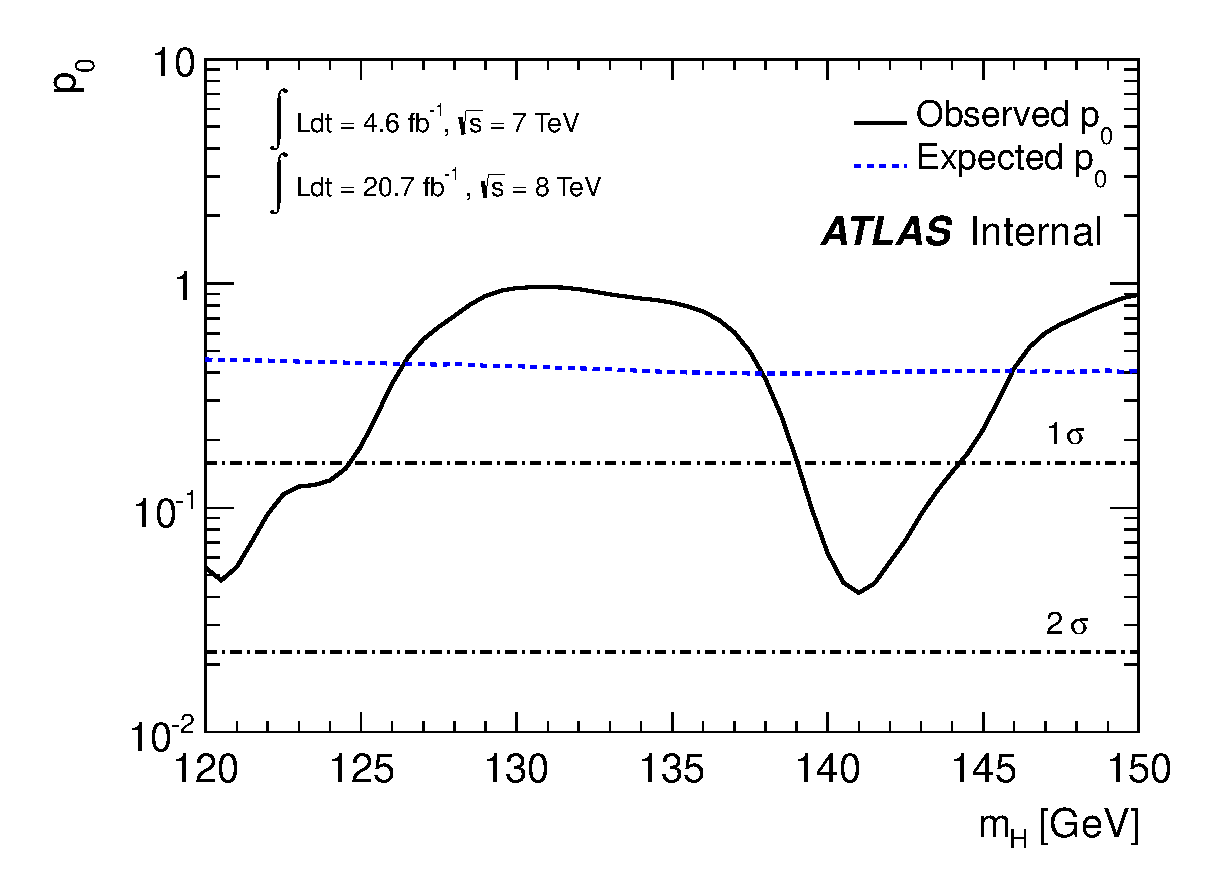
\includegraphics[totalheight=9cm,angle=0]{figures/plot_p0}}
    \caption{Expected (dashed blue line) and observed 
      (solid black line) $p_0$ (compatibility of
      the data with the background-only hypothesis) as a function
      of the Higgs boson mass, using \lumiseventev~\ifb\ of $pp$
      collisions at $\sqrt{s}=7$~TeV and \lumieighttev~\ifb\ of $pp$
      collisions at $\sqrt{s}=8$~TeV.}
    \label{fig:ExpectedP0_1}
\end{figure}

Subsequently, upper limits on the production cross-section of \HToZg are set.
Both observed limits, computed using real data, and expected limits, computed using
Asimov dataset generated with the $\mu=0$ hypothesis are shown in 
\refF{fig:ExpectedExclusion_1}. The expected 95\% $CL_s$ limit ranges between
7.3 and 22 and the observed one varies between 5.4 and 37 for a Higgs boson
mass between 120 and 150 GeV. In particular, for a mass of 125 GeV, consistent
with the mass of the recently discovered Higgs-like boson, the expect and observed
limits are equal to 13.5 and 18.2 times the Standard Model, respectively. The
results are dominated by the statistical uncertainties.

\begin{figure}[!htbp]
\centering
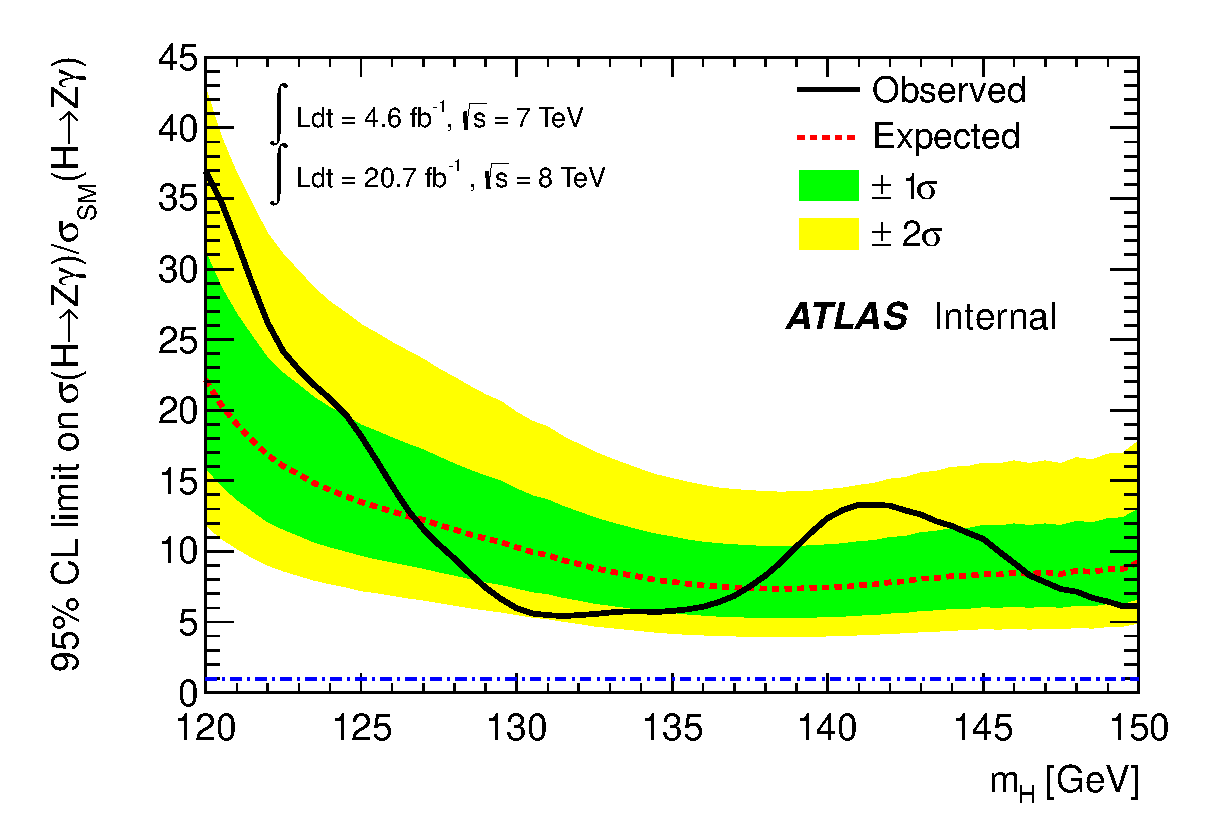
\includegraphics[totalheight=9cm,angle=0]{figures/plot_smooth_cls}
\caption{Observed 95\% $CL$ limits (solid black line) 
  on the production cross section of a SM Higgs boson 
  decaying to $Z\gamma$, as a function of the Higgs boson 
  mass, using \lumiseventev~\ifb\ of $pp$
  collisions at $\sqrt{s}=7$~TeV and \lumieighttev~\ifb\ of $pp$
  collisions at $\sqrt{s}=8$~TeV.
  The median expected 95\% $CL$ exclusion limits (dashed red line)
  are also shown. The green and yellow bands correspond to the $\pm 1\sigma$ 
  and $\pm2\sigma$ intervals.
}
\label{fig:ExpectedExclusion_1}
\end{figure}
